\section{Time Domain Reflectometry}

\subsection{Measurement A: Rise- and fall time of the line driver}

\subsubsection{Task Description}
The rise and fall times of the signal generator and the open output of the line driver were measured. The line driver (LM5134 and LMG1025) was supplied with +5 V. The function generator was configured to output a rectangular signal with 5 Vpp and a 2.5 V DC offset.

\subsubsection{Schematic}
The measurement setup utilizes an Arbitrary Waveform Generator connected to the line driver input. The driver output connects to an SMA connector via two 2.7 Ω series resistors (5.4 Ω total series resistance). A 1 kΩ resistor connected to a second SMA forms a 1:21 voltage divider in combination with the 50 Ω input of the oscilloscope and the coaxial line.  For this measurement, the output coaxial line and the load ZL were left disconnected to simulate an open driver output, as illustrated in Figure 2.1.  

\begin{figure}[htpb]
    \centering
    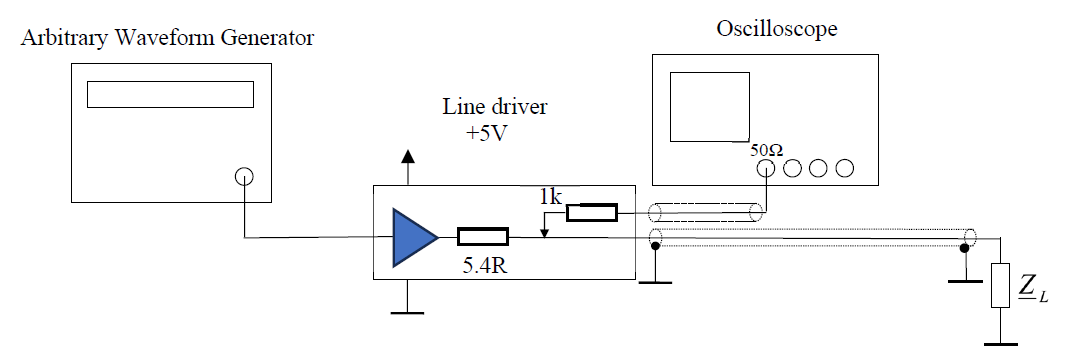
\includegraphics[width=\textwidth]{src/figers/ex_2/Schematic.png}
    \caption{General measurement setup for Time Domain Reflectometry showing the AWG, line driver, 1:21 voltage divider, oscilloscope, coaxial line, and termination load $\underline{Z}_L$.}
    \label{fig:schematic}
\end{figure}

\subsubsection{Formulas and Calculations}

Rise and fall times were determined using the oscilloscope's automatic measurement functions. No calculations were required for this measurement.

\subsubsection{Measurement results}

\begin{table}[ht!]
    \centering
    \begin{tabular}{|c|c|c|c|}
        \hline
        \textbf{Adjusted} & \textbf{Measured} & \textbf{Measured} & \textbf{Calculated} \\
        \hline
        Test Point & Rise Time $t_r$ / ns & Fall Time $t_f$ / ns & - \\
        \hline
        Signal Generator & 8.354 & 4.374 & - \\
        \hline
        Line Driver (Open Output) & 1.282 & Not measured* & - \\
        \hline
    \end{tabular}
    \caption{\centering Rise and fall times of the signal generator and line driver. Notes: Function generator set to 5 V$_{\text{pp}}$, 2.5 V DC offset. *Fall time for the line driver could not be evaluated.}
    \label{tab:rise_fall_times}
\end{table}
\FloatBarrier

\subsubsection{Curves \& diagrams}

\begin{figure}[htpb]
    \centering
    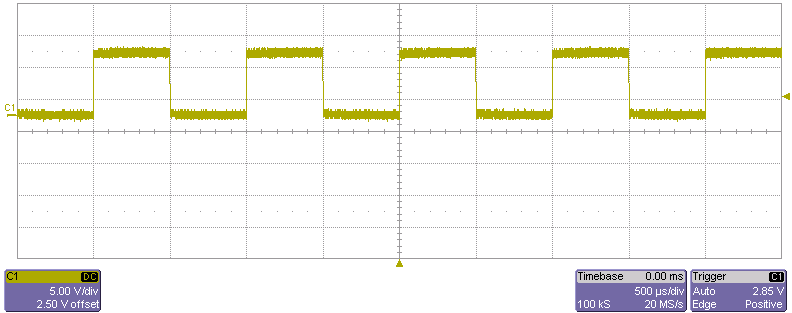
\includegraphics[width=0.8\textwidth]{src/figers/ex_2/sinewave.png}
    \caption{Rectangular input signal from the Arbitrary Waveform Generator (5 V$_{\text{pp}}$, 2.5 V DC offset).}
    \label{fig:awg_input}
\end{figure}

\begin{figure}[htpb]
    \centering
    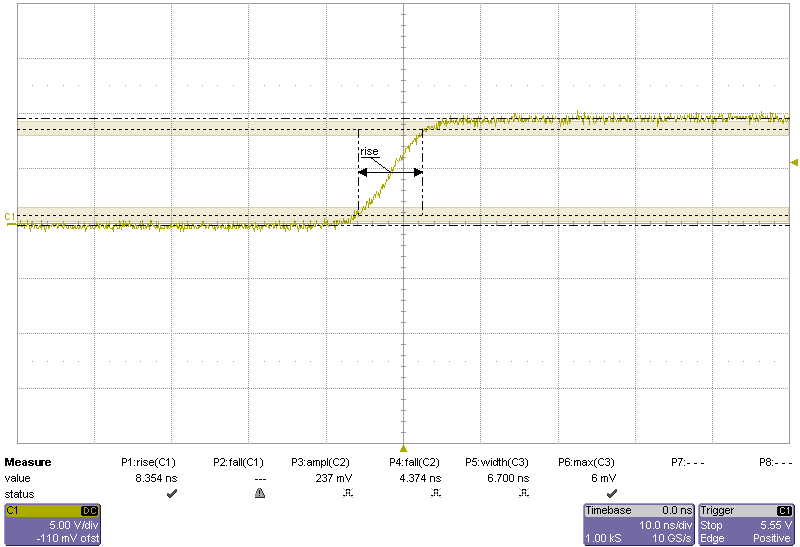
\includegraphics[width=0.8\textwidth]{src/figers/ex_2/risetime_sinewave.png}
    \caption{Transient voltage curve showing the rise and fall time measurements of the signal generator.}
    \label{fig:risetime_generator}
\end{figure}

\begin{figure}[htpb]
    \centering
    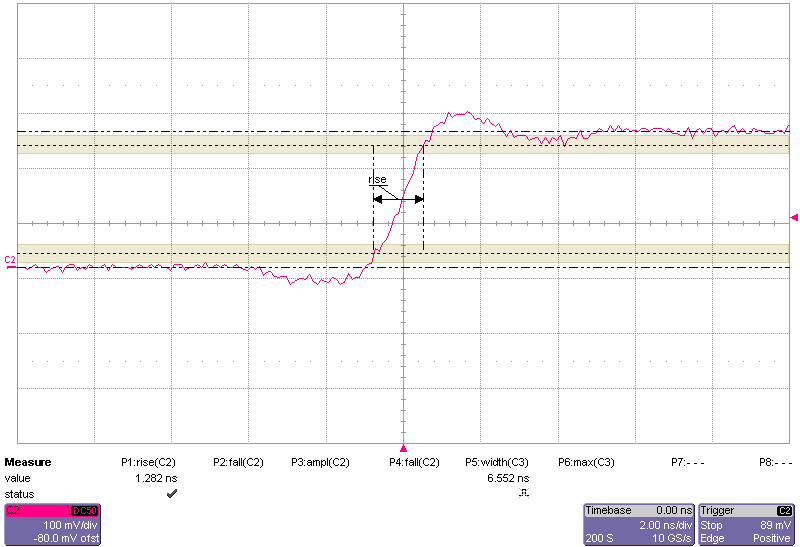
\includegraphics[width=0.8\textwidth]{src/figers/ex_2/risetime_gatedrivers.png}
    \caption{Transient voltage curve showing the much steeper rise time at the open output of the line driver.}
    \label{fig:risetime_driver}
\end{figure}
\FloatBarrier

\subsubsection{Short discussion of measurement results}

The line driver significantly steepens the signal edge. The signal generator alone has a rise time of 8.354 ns and a fall time of 4.374 ns. The LM5134 and LMG1025 gate drivers reduce this rise time to 1.282 ns. This fast transition is necessary for TDR to provide high spatial resolution when separating incident and reflected waves.  The fall time at the driver output could not be captured. With a ~1 kHz input signal, the falling edge occurs roughly 500 µs after the rising edge. Because the oscilloscope timebase was set to 2.00 ns/div to measure the nanosecond rise time, the falling edge fell completely outside the acquisition window.

\subsection{Measurement B: Reflections of a coax cable with different loads}

\subsubsection{Task Description}
A 2.0 m RG142 coaxial cable was connected to the line driver output (see Figure 2.1). The cable was terminated with various load impedances $Z_L$ (Open, Short, 50 Ω, 100 Ω, 25 Ω, 100 pF, and 1 nH). Transient voltage curves were recorded to measure the time delay between reflections, the maximum voltage, and the steady-state asymptotic voltage. From the measured propagation delay and physical cable length, the relative dielectric constant ($\epsilon_r$) of the cable was calculated.  

\subsubsection{Formulas and Calculations}

The reflection factor $\rho_0$ at the load is determined by the load impedance $Z_L$ and the characteristic impedance $Z_w$ of the transmission line:

\begin{equation}
    \rho_0 = \frac{Z_L - Z_w}{Z_L + Z_w}
\end{equation}

The phase velocity $v_p$ of the signal propagating through the transmission line depends on the speed of light in a vacuum ($c = 2.9979 \times 10^8$ m/s) and the relative dielectric constant $\epsilon_r$:

\begin{equation}
    v_p = \frac{c}{\sqrt{\epsilon_r}}
\end{equation}

The time delay $t$ measured between the incident wave and the reflected wave represents the round trip of the signal along the length of the cable $l$:

\begin{equation}
    t = \frac{2l}{v_p}
\end{equation}

By substituting the phase velocity formula into the time delay formula, the dielectric constant $\epsilon_r$ can be calculated from the physical length and the measured time delay:

\begin{equation}
    \epsilon_r = \left( \frac{c \cdot t}{2l} \right)^2
\end{equation}

Exemplary Calculation:

To demonstrate the calculation process for the values populated in the "calculated" columns of the measurement table, the 100 $\Omega$ load and Open circuit measurements are evaluated below.

For a characteristic impedance of $Z_w = 50\ \Omega$ and a load of $Z_L = 100\ \Omega$, the reflection factor is calculated as:

\begin{equation}
    \rho_0 = \frac{100\ \Omega - 50\ \Omega}{100\ \Omega + 50\ \Omega} = \frac{50}{150} = +0.33
\end{equation}

For the Open load measurement, a time delay of $t = 19.6$ ns was recorded across the $l = 2.0$ m cable. The relative dielectric constant is calculated as:

\begin{equation}
    \epsilon_r = \left( \frac{2.9979 \times 10^8\ \text{m/s} \cdot 19.6 \times 10^{-9}\ \text{s}}{2 \cdot 2.0\ \text{m}} \right)^2 = \left( \frac{5.875}{4.0} \right)^2 \approx 2.16
\end{equation}

\subsubsection{Measurement results}

\begin{table}[ht!]
    \centering
    \resizebox{\textwidth}{!}{%
    \begin{tabular}{|c|c|c|c|c|c|}
        \hline
        \textbf{Adjusted} & \textbf{Measured} & \textbf{Measured} & \textbf{Measured} & \textbf{Calculated} & \textbf{Calculated} \\
        \hline
        Load $Z_L$ & Time Delay $t$ / ns & Max Voltage $V_{\text{max}}$ / mV & Steady-state Voltage $V_{\text{steady}}$ / mV & Reflection Factor $\rho_0$ & Dielectric Const. $\epsilon_r$ \\
        \hline
        Open & 19.6 & 300 & 300 & +1 & 2.16 \\
        \hline
        Short & 19.6 & 150 & 0 & -1 & 2.16 \\
        \hline
        50 $\Omega$ & 19.5 & 150 & 150 & 0 & 2.14 \\
        \hline
        100 $\Omega$ & 19.5 & 200 & 200 & +0.33 & 2.14 \\
        \hline
        25 $\Omega$ & 19.5 & 150 & 100 & -0.33 & 2.14 \\
        \hline
        100 pF & 19.7 & 300 & 300 & $\rightarrow$ +1 (transient) & 2.18 \\
        \hline
        1 nH & 21.3 & 300 & 0 & $\rightarrow$ -1 (transient) & 2.55 \\
        \hline
    \end{tabular}%
    }
    \caption{\centering Reflection characteristics and calculated parameters for various loads. Notes: Physical length of RG142 cable $l = 2.0$ m. Characteristic impedance $Z_w = 50\ \Omega$. Voltage values represent raw oscilloscope readings measured via the 1:21 voltage divider (incident wave $V_{\text{inc}} \approx 150$ mV). For reactive loads, $\rho_0$ denotes the final steady-state reflection factor. The average calculated $\epsilon_r$ for the resistive loads is 2.15.}
    \label{tab:reflections_different_loads}
\end{table}
\FloatBarrier

\subsubsection{Curves \& diagrams}

\begin{figure}[htpb]
    \centering
    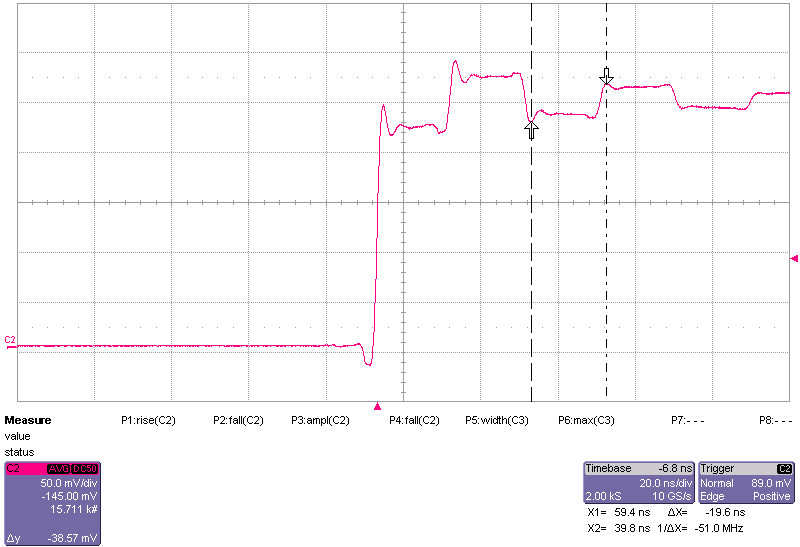
\includegraphics[width=0.8\textwidth]{src/figers/ex_2/refl_open.png}
    \caption{Transient voltage curve for an open-ended transmission line.}
    \label{fig:refl_open}
\end{figure}

\begin{figure}[htpb]
    \centering
    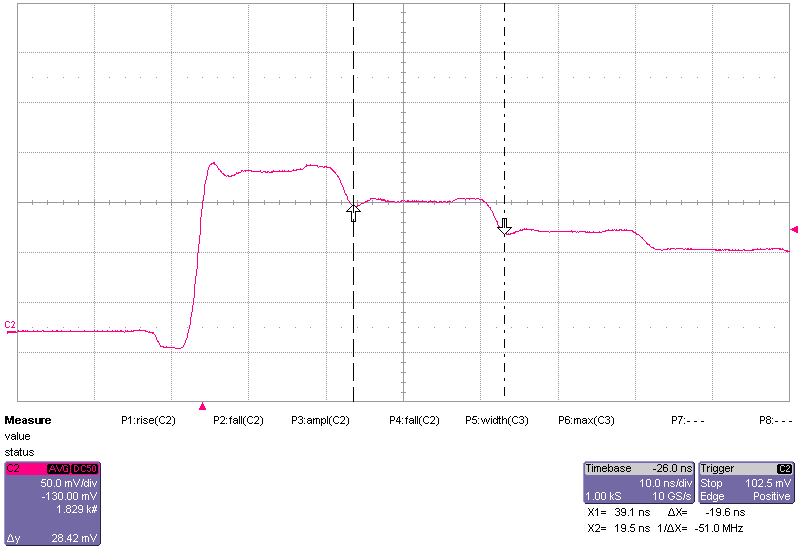
\includegraphics[width=0.8\textwidth]{src/figers/ex_2/refl_short.png}
    \caption{Transient voltage curve for a short-circuited transmission line.}
    \label{fig:refl_short}
\end{figure}

\begin{figure}[htpb]
    \centering
    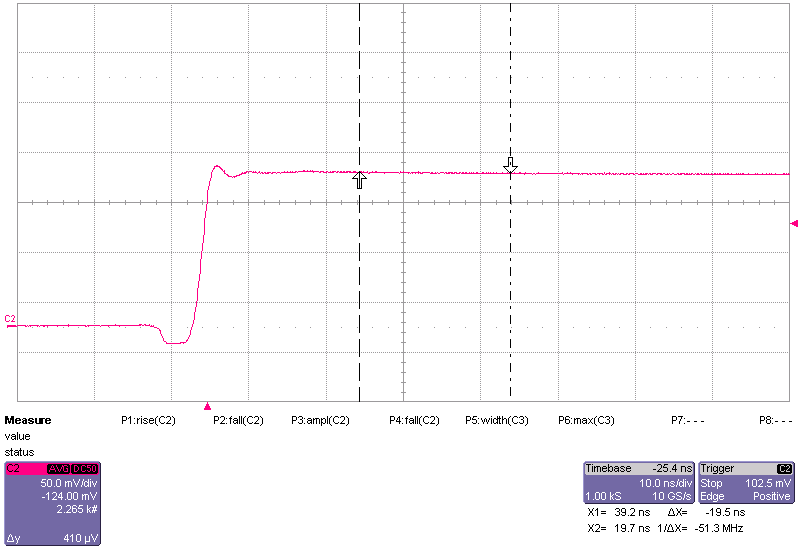
\includegraphics[width=0.8\textwidth]{src/figers/ex_2/refl_50ohm.png}
    \caption{Transient voltage curve for a matched 50 $\Omega$ load.}
    \label{fig:refl_50ohm}
\end{figure}

\begin{figure}[htpb]
    \centering
    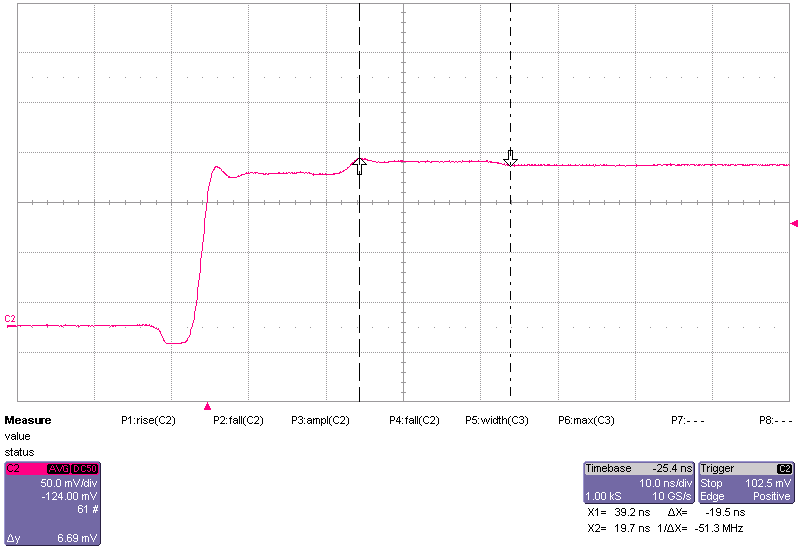
\includegraphics[width=0.8\textwidth]{src/figers/ex_2/refl_100ohm.png}
    \caption{Transient voltage curve for a 100 $\Omega$ load.}
    \label{fig:refl_100ohm}
\end{figure}

\begin{figure}[htpb]
    \centering
    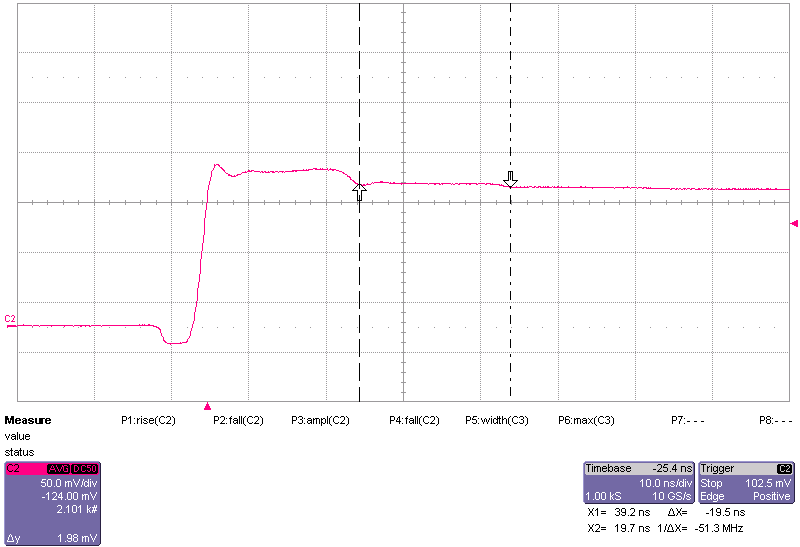
\includegraphics[width=0.8\textwidth]{src/figers/ex_2/refl_25ohm.png}
    \caption{Transient voltage curve for a 25 $\Omega$ load.}
    \label{fig:refl_25ohm}
\end{figure}

\begin{figure}[htpb]
    \centering
    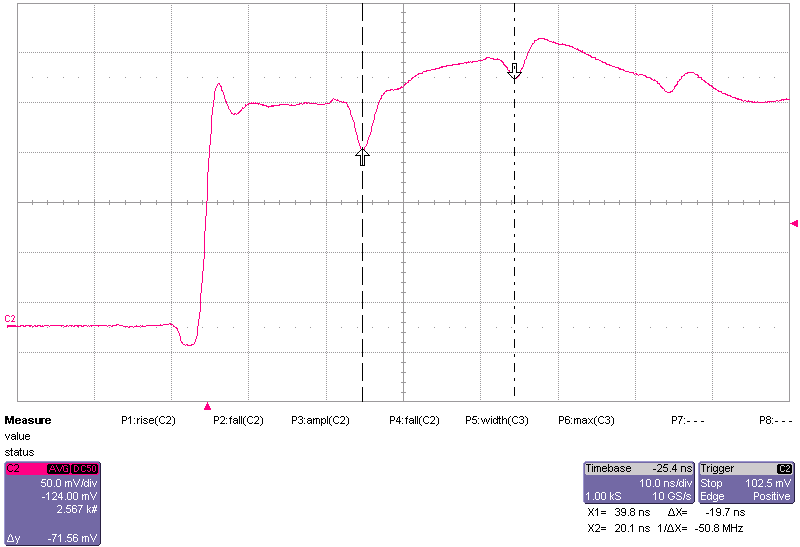
\includegraphics[width=0.8\textwidth]{src/figers/ex_2/refl_100pF_cap.png}
    \caption{Transient voltage curve for a 100 pF capacitive load.}
    \label{fig:refl_100pF_cap}
\end{figure}

\begin{figure}[htpb]
    \centering
    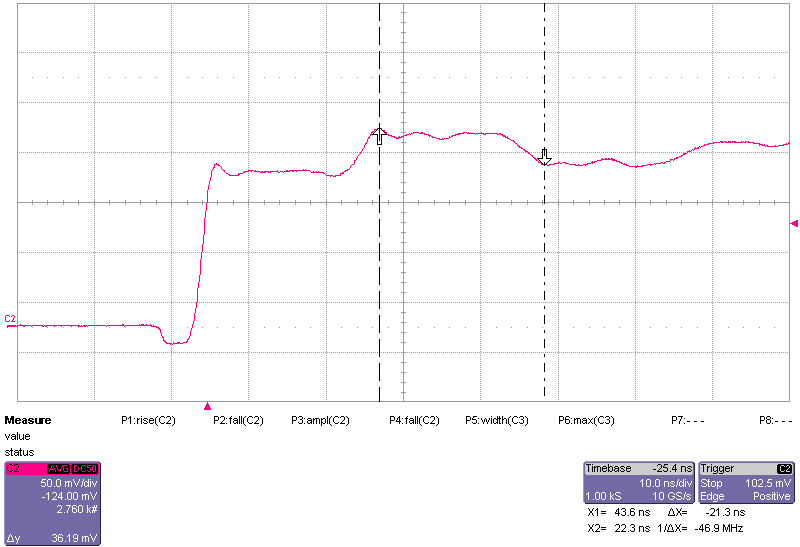
\includegraphics[width=0.8\textwidth]{src/figers/ex_2/refl_1nH_inductor.png}
    \caption{Transient voltage curve for a 1 nH inductive load.}
    \label{fig:refl_1nH_inductor}
\end{figure}
\FloatBarrier

\subsubsection{Short discussion of measurement results}

The measured transient responses match standard transmission line behavior. The incident voltage step ($V_{\text{inc}}$) was approximately 150 mV on the oscilloscope, corresponding to a 3.15 V line voltage before the 1:21 divider.

\begin{itemize}
    \item \textbf{Open Circuit:} The positive reflection ($\rho_0 = +1$) doubled the incident voltage to a maximum of 300 mV.
    \item \textbf{Short Circuit:} The negative reflection ($\rho_0 = -1$) canceled the voltage at the load, dropping it to 0 mV.
    \item \textbf{Matched Load (50 $\Omega$):} With $\rho_0 = 0$, no backward wave was generated, and the voltage remained constant at 150 mV.
    \item \textbf{100 $\Omega$ and 25 $\Omega$ Loads:} The 100 $\Omega$ load produced a partial positive reflection (+50 mV), settling at 200 mV. The 25 $\Omega$ load produced a partial negative reflection (-50 mV), settling at 100 mV.
    \item \textbf{100 pF Capacitor:} Initially acted as a short circuit during the signal step, then charged towards an open-circuit steady state ($\rho_0 \rightarrow +1$).
    \item \textbf{1 nH Inductor:} Initially acted as an open circuit (producing a 300 mV peak), then settled into a short-circuit steady state ($\rho_0 \rightarrow -1$).
\end{itemize}

\vspace{1em}
\noindent\textbf{Time Delay and Dielectric Constant}

The time delay across the purely resistive, open, and short loads averaged 19.55 ns.

For the 2.0 m RG142 cable, the resulting relative dielectric constant ($\epsilon_r$) is 2.15. This aligns with the theoretical permittivity of its PTFE dielectric ($\epsilon_r \approx 2.1$).

The delay for the 1 nH inductor deviated slightly ($\Delta t = 21.3$ ns). This is due to the higher reading error when placing cursors on a rounded transient slope rather than a sharp step.

\subsection{Measurement C: Determine cable length}

\subsubsection{Task Description}
The physical length of an unknown RG58 coaxial cable was determined by measuring its TDR propagation delay. The relative dielectric constant ($\epsilon_r$) calculated in Measurement B was used for this calculation.

The RG142 cable in the setup (Figure 2.1) was replaced with the open-ended RG58 cable.

\subsubsection{Formulas and Calculations}

Using the time delay $t$ measured from the oscilloscope and the phase velocity $v_p$ (derived from the $\epsilon_r$ calculated in Measurement B), the unknown length $l$ of the cable can be calculated by rearranging the time delay formula:

\begin{equation}
    l = \frac{v_p \cdot t}{2} = \frac{c \cdot t}{2\sqrt{\epsilon_r}}
\end{equation}

Exemplary Calculation:

To demonstrate the calculation process for the value populated in the "calculated" column of the measurement table, the length of the unknown RG58 cable is evaluated below.

Given the speed of light in a vacuum $c = 2.9979 \times 10^8$ m/s, the adopted average relative dielectric constant $\epsilon_r = 2.15$ (from Measurement B), and the measured time delay $t = 12.0$ ns, the physical length $l$ of the cable is calculated as:

\begin{equation}
    l = \frac{2.9979 \times 10^8\ \text{m/s} \cdot 12.0 \times 10^{-9}\ \text{s}}{2\sqrt{2.15}} = \frac{3.5975\ \text{m}}{2 \cdot 1.466} \approx 1.23\ \text{m}
\end{equation}

\subsubsection{Measurement results}

\begin{table}[ht!]
    \centering
    \begin{tabular}{|c|c|c|}
        \hline
        \textbf{Adjusted} & \textbf{Measured} & \textbf{Calculated} \\
        \hline
        Assumed $\epsilon_r$ & Time Delay $t$ / ns & Calculated Length $l$ / m \\
        \hline
        2.15 & 12.0 & 1.23 \\
        \hline
    \end{tabular}
    \caption{\centering Determination of the unknown RG58 cable length. Notes: The relative dielectric constant $\epsilon_r = 2.15$ is adopted from the RG142 measurements as per lab instructions. The true physical length of the cable was later measured to be exactly 1.20 m.}
    \label{tab:rg58_length}
\end{table}
\FloatBarrier

\subsubsection{Curves \& diagrams}

\begin{figure}[htpb]
    \centering
    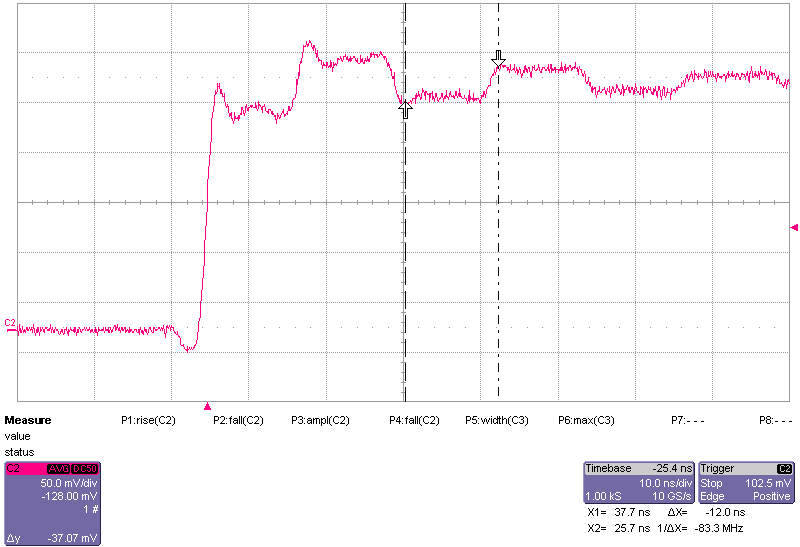
\includegraphics[width=0.8\textwidth]{src/figers/ex_2/refl_cable_len.png}
    \caption{Transient voltage curve showing the time delay measurement for the unknown RG58 coaxial cable.}
    \label{fig:refl_cable_len}
\end{figure}
\FloatBarrier

\subsubsection{Short discussion of measurement results}

\begin{itemize}
    \item A positive reflection confirmed the RG58 cable was open-ended. The round-trip time delay was measured at 12.0 ns.
    \item Using $\epsilon_r = 2.15$ from Measurement B, the calculated cable length is 1.23 m. The measured physical length was 1.20 m, resulting in a 3 cm overestimation.
    \item This deviation is a systematic error caused by applying the PTFE dielectric constant of the RG142 cable to the polyethylene RG58 cable.
    \item Standard RG58 cables have a relative permittivity of $\epsilon_r = 2.26$. Recalculating with this value yields 1.196 m, which is within 4 mm of the physical measurement.
\end{itemize}